\section{Image Processing Operations}
The \textit{CryptoImg} library implemented several
We discuss two basic types of image processing operations, \textit{intensity transformations}, which map an intensity value to another, and \textit{spatial filters} which consider intensity values from regions of pixels to perform operations such as edge detection, image blurring and sharpening.

We represent a digital image $R$ as an $M \times N$ matrix of pixel intensity values, each value in the range $\left[0, L-1\right]$, for some positive integer $L$. We use $R(x,y)$ represents the entry at the $x$th row and $y$th column of a matrix $R$.

\subsection{Intensity Transformations}
An Intensity transformation on an image $R$ can be defined as a function $T$ which maps a pixel value $r$ to a new value $r^\prime$, which we can write as $r^\prime = T\left(r\right)$. This function is then applied to every pixel in $R$.

The \textit{CryptoImg} library implemented two types of linear intensity transformations: image negation and brightness control.
An image negation transformation is defined as:
\begin{equation}
    T\left(r\right) = L-1-r
\end{equation}
After applying image negation, the resulting image would be similar to a photographic negative~\cite{gonzalez_digital_2008}.

A brightness control transformation with parameter $v$ is defined as:
\begin{equation}
    T\left(r,v\right) = r+v
\end{equation}
The above transformations are linear in terms of the input $r$, and are thus simple to implement under a homomorphic cryptosystem.

In this study we extend the range of intensity transformations to non-linear transformations. Two common non-linear image transformations are the log transformation and power-law transformation~\cite{gonzalez_digital_2008}.

The log transformation is used to enhance dark pixels or increase the dark details of an image by mapping low intensity values to a wider range of values~\cite{gonzalez_digital_2008}. This has the general formula
\begin{equation}
    T\left(r\right) = c \log\left(1 + r\right)
\end{equation}
where $c$ is a constant.

The power-law transformation is a family of transformations that have the form
\begin{equation}
    T\left(r\right) = c r^{\gamma}
\end{equation}
where $c>0$ and $\gamma > 0$.
A power-law transformation defined by the above equation can calibrate the operation of many image capture and output devices such as cameras, printers and displays in a process called \textit{gamma correction}. This ensures reproducibility and accuracy of images being displayed by digital output devices~\cite{gonzalez_digital_2008}.

To implement non-linear intensity transformations using addition and multiplication in a homomorphic system, it is necessary to approximate the logarithm and exponential functions, which may result in higher computational overhead. In our software library implementation, we investigate methods required to approximate the logarithm and functions.

\subsection{Spatial Filtering}
The \textit{CryptoImg} library also implemented \textit{spatial filters}. Spatial filters are operators which determine output pixels using information from neighboring input pixels. To apply a spatial filter to obtain a resulting image $R^\prime$, a convolution is performed between an $m \times n$ matrix $k$, called a kernel, and the original $M\times N$ image $R$.
A convolution between a kernel $k$ and image $R$ which yields a resulting image $R^\prime$, denoted as $R^\prime = k \ast R$, is defined by
\begin{align} \label{eq:spatialfilter}
	R^\prime(x,y) = \sum_{s=1}^m{\sum_{t=1}^n{k(s,t)R(x+s,y+t)}}, \text{ for all } 0\leq x \leq M, 0 \leq y \leq N,
\end{align}

\begin{figure*}[!ht]
    \centering
    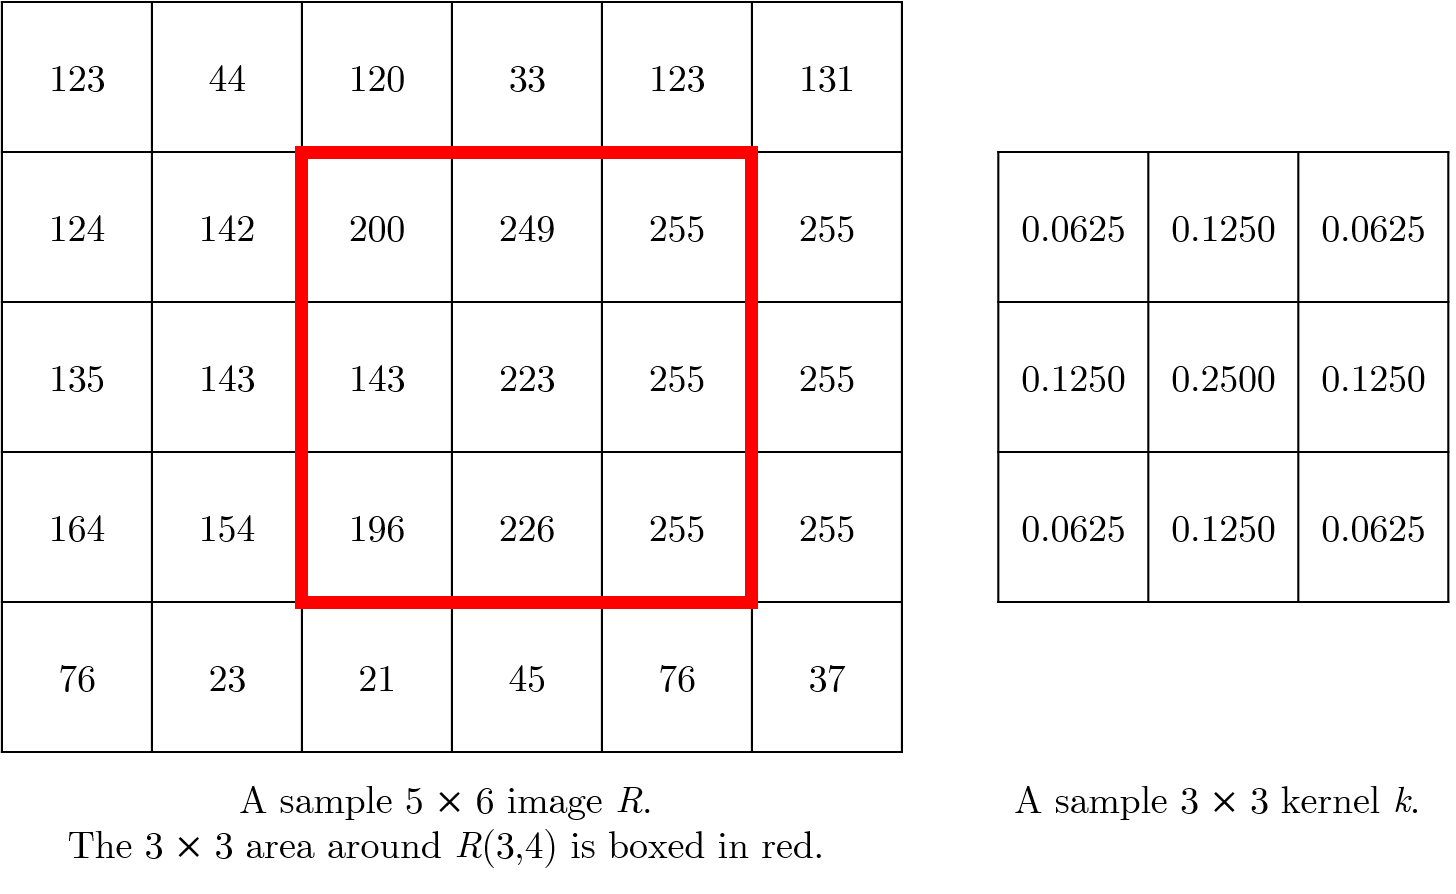
\includegraphics[width=\textwidth,\keepaspectratio]{Figures/SpatialFilter.png}
    \caption{A sample image $R$ and sample kernel $k$.}
    \label{fig:spatialfilter}
\end{figure*}
For example, using the image and $3 \times 3$ kernel given in Figure \ref{fig:spatialfilter}, we can calculate the value in the third row and fourth column of the resulting image $R^\prime$ by adding the products of entries in $k$ with the corresponding entries in $R$, found in an $3 \times 3$ region around $R(3,4)$.
\begin{align*}
	R^\prime(3,4) &= \sum_{s=1}^m{\sum_{t=1}^n{k(s,t)R(3+s,4+t)}}\\
	&= (0.0625\times 200) + (0.1250\times 249) + (0.0625\times 255) \\
	&+ (0.1250\times 143) + (0.2500\times 223) + (0.1250\times 255) \\
	&+ (0.0625\times 196) + (0.1250\times 236) + (0.0625\times 255)\\
	&= 223.
\end{align*}
Since spatial filters take values from a contiguous region of pixels, this presents a difficulty in homomorphic cryptosystems: in order for spatial filters to be performed, the location of each pixel relative to neighboring pixels has to be preserved. This was performed in the implementation of spatial filters in the \textit{CryptoImg} library~\cite{ziad_cryptoimg:_2016}. We wish to implement spatial filters using a similar approach, and assess how preserving spatial correlation between pixels can impact the security of the encrypted image.

\subsection{Common Spatial Filtering Kernels}
Edge detection is used to find and determine the boundaries in an image, commonly used in applications such as image segmentation and feature extraction. This works by detecting so-called \textit{edges}, areas that have abrupt changes in intensity.
One common method of performing edge detection is the Sobel operator, which uses two spatial filters to approximate the gradient of an image. Given an image $R$, and the kernels
\begin{equation}
    g_x =
    \begin{bmatrix}
        -1 & 0 & 1 \\
        -2 & 0 & 2 \\
        -1 & 0 & 1
    \end{bmatrix}
    \qquad\text{and}\qquad
    g_y =
    \begin{bmatrix}
        1 & 2 & 1 \\
        0 & 0 & 0 \\
        -1 & -2 & -1
    \end{bmatrix},
\end{equation}
$g_x \ast R$ yields the horizontal component of the gradient, while $g_y \ast R$ yields the vertical component of the gradient.

There are also spatial filters that perform image smoothing (such as Gaussian blur and box blur, which use the kernels $b_g$ and $b$ respectively in Equation~\ref{eqn:smooth-filters}) and image sharpening~\cite{gonzalez_digital_2008}.
\begin{equation}
    \label{eqn:smooth-filters}
    b_g = \frac{1}{16}
    \begin{bmatrix}
        1 & 2 & 1 \\
        2 & 4 & 2 \\
        1 & 2 & 1
    \end{bmatrix}
    \qquad
    b = \frac{1}{9}
    \begin{bmatrix}
        1 & 1 & 1 \\
        1 & 1 & 1 \\
        1 & 1 & 1
    \end{bmatrix}
\end{equation}

%% TODO: specific list of kernels to use for this study
